\section{Usefull keyword and concepts remarks}
\label{sec:Useufull-keyword-remarks}
%~\cref{sec:Useufull-keyword-remarks}
\subsection{Predicate and utility functions}
\label{subsec:Keyword auto}
%~\cref{subsec:Useufull-keyword-remarks-00-fcn-predicate-utility}
A \textbf{predicate function} (also known as \textbf{access function}) are basically functions that can read or display data. Also functions thatn can be read and serves to test the truth or falsity of conditions.\\

\noindent A \textbf{utility function} (also known as helper function) is a \CppKeywordCommon{private} member function that supports the operation of the class\textquotesingle{}\,s \CppKeywordCommon{public} member functions, but is \underline{not} intended for use by clients of the class


\subsection{Keyword \texttt{auto}}
\label{subsec:Keyword auto}
%~\cref{subsec:Useufull-keyword-remarks-01-Keyword-auto}
One of the most important advantage of using \CppKeywordCommon{auto} is that you need to initialize the variable. Normally you can track your type and also deduce your type. 
\begin{itemize}
    %%%%%%%%%%%%%%%%%%%%%%%%%%%%%%%%%%%%%%%%%% ITEM 
    \item To make th type track, deduce:\\
    \begin{minipage}{\MPWxXXSxLISTING\textwidth} % = 0.7 times \textwidth
    \vspaceTextToListing % =\vspace{0.1cm}
        \begin{CPPCode}
auto var = init;
        \end{CPPCode}
    \end{minipage}\\ 
    Example given:\\
\begin{minipage}{\MPWxXXSxLISTING\textwidth} % = 0.7 times \textwidth
\vspaceTextToListing % =\vspace{0.1cm}
        \begin{CPPCode}
//old style:
const char* s = "Hello";
widget w = get_widget();
        \end{CPPCode}
    \end{minipage}
    \hspaceListingXSToListingXS
    \begin{minipage}{\MPWxXXSxLISTING\textwidth} % = 0.7 times \textwidth
    \vspaceTextToListing
        \begin{CPPCode}
//better style:
auto s = "Hello";
auto w = get_widget();
        \end{CPPCode}
    \end{minipage}
    %%%%%%%%%%%%%%%%%%%%%%%%%%%%%%%%%%%%%%%%%% ITEM 
    \item To make type stick, commit:\\
    \begin{minipage}{\MPWxXXSxLISTING\textwidth} % = 0.7 times \textwidth
\vspaceTextToListing % =\vspace{0.1cm}
        \begin{CPPCode}
        auto var = type{ init };
\end{CPPCode}
\end{minipage}\\
 \begin{minipage}{\MPWxXXSxLISTING\textwidth} % = 0.7 times \textwidth
\vspaceTextToListing % =\vspace{0.1cm}
\begin{CPPCode}
        type var{ init };
\end{CPPCode}
    \end{minipage}\\
    Example given:\\
\begin{minipage}{\MPWxXXSxLISTING\textwidth} % = 0.7 times \textwidth
\vspaceTextToListing % =\vspace{0.1cm}
        \begin{CPPCode}
//old style:
employee e{ empid };
widget w{ 12, 34};
        \end{CPPCode}
    \end{minipage}
    \hspaceListingXSToListingXS
    \begin{minipage}{\MPWxXXSxLISTING\textwidth} % = 0.7 times \textwidth
    \vspaceTextToListing
        \begin{CPPCode}
//better style:
auto e = employee{ empid };
auto w = widget{ 12, 34};
        \end{CPPCode}
    \end{minipage}
    
    %%%%%%%%%%%%%%%%%%%%%%%%%%%%%%%%%%%%%%%%%% ITEM 
    \item With heap allocation, type is on the right naturally anyway\\
    \begin{minipage}{\MPWxXXSxLISTING\textwidth} % = 0.7 times \textwidth
\vspaceTextToListing % =\vspace{0.1cm}
        \begin{CPPCode}
auto w = new widget{}           
auto w = make_unique<widget>();
        \end{CPPCode}
    \end{minipage}
    \hspaceListingXSToListingXS
    \begin{minipage}{\MPWxXXSxLISTING\textwidth} % = 0.7 times \textwidth
    \vspaceTextToListing
        \begin{CPPCode}
C++98 Style
C++14 Style
        \end{CPPCode}
    \end{minipage}

    %%%%%%%%%%%%%%%%%%%%%%%%%%%%%%%%%%%%%%%%%% ITEM 
    \item However, what about \CppKeywordCommon{int} vs \CppKeywordCommon{auto} ?\\
        \begin{minipage}{\MPWxXXSxLISTING\textwidth} % = 0.7 times \textwidth
\vspaceTextToListing % =\vspace{0.1cm}
        \begin{CPPCode}
int x = 42;
        \end{CPPCode}
    \end{minipage}
    \hspaceListingXSToListingXS
    \begin{minipage}{\MPWxXXSxLISTING\textwidth} % = 0.7 times \textwidth
    \vspaceTextToListing
        \begin{CPPCode}
auto = 42;
        \end{CPPCode}
    \end{minipage}

    %%%%%%%%%%%%%%%%%%%%%%%%%%%%%%%%%%%%%%%%%% ITEM 
    \item Well there are two arguments: consistency, and no narrowing. Additionally, you can use literal suffixes\\
    \begin{minipage}{\MPWxXXSxLISTING\textwidth} % = 0.7 times \textwidth
\vspaceTextToListing % =\vspace{0.1cm}
        \begin{CPPCode}
employee e{ empid };
widget w{ 12, 34};
int x = 42;
float x = 42;
unsigned long x = 42;
string x = "42";
chrono::nanoseconds x{42}
        \end{CPPCode}
    \end{minipage}
    \hspaceListingXSToListingXS
    \begin{minipage}{\MPWxXXSxLISTING\textwidth} % = 0.7 times \textwidth
    \vspaceTextToListing
        \begin{CPPCode}
auto e = employee{ empid };
auto w = widget{ 12, 34};
auto x = 42;
auto x = 42.f;       //lit. suffix
auto x = 42.ul; //lit. suffix
auto x = "42"s  //C++14
auto x = 42ns       //C++14
        \end{CPPCode}
    \end{minipage}

    %%%%%%%%%%%%%%%%%%%%%%%%%%%%%%%%%%%%%%%%%% ITEM 
    \item In function declaration and named lambdas( 1st and 2nd row respec.):\\
    \begin{minipage}{\MPWxXXSxLISTING\textwidth} % = 0.7 times \textwidth
\vspaceTextToListing % =\vspace{0.1cm}
        \begin{CPPCode}
int f( double )

        \end{CPPCode}
    \end{minipage}
    \hspaceListingXSToListingXS
    \begin{minipage}{\MPWxXXSxLISTING\textwidth} % = 0.7 times \textwidth
    \vspaceTextToListing
        \begin{CPPCode}
auto f (double) -> int;
auto f = [=](double) { /*... */ }
        \end{CPPCode}
    \end{minipage}

    %%%%%%%%%%%%%%%%%%%%%%%%%%%%%%%%%%%%%%%%%% ITEM 
    \item Aliases (no more typedefs)\\
    \begin{minipage}{\MPWxXXSxLISTING\textwidth} % = 0.7 times \textwidth
\vspaceTextToListing % =\vspace{0.1cm}
        \begin{CPPCode}
typedef set<string>dict;
        \end{CPPCode}
    \end{minipage}
    \hspaceListingXSToListingXS
    \begin{minipage}{\MPWxXXSxLISTING\textwidth} % = 0.7 times \textwidth
    \vspaceTextToListing
        \begin{CPPCode}
using dict = set<string>;
        \end{CPPCode}
    \end{minipage}

    %%%%%%%%%%%%%%%%%%%%%%%%%%%%%%%%%%%%%%%%%% ITEM 
    \item Template aliases\\
    \begin{minipage}{\MPWxXXSxLISTING\textwidth} % = 0.7 times \textwidth
\vspaceTextToListing % =\vspace{0.1cm}
        \begin{CPPCode}
template<class T>struct myvec
{typedef vector<T,myalloc> type;}
        \end{CPPCode}
    \end{minipage}
    \hspaceListingXSToListingXS
    \begin{minipage}{\MPWxXXSxLISTING\textwidth} % = 0.7 times \textwidth
    \vspaceTextToListing
        \begin{CPPCode}
template<class T>
using myvec = vector<T,myalloc>;
        \end{CPPCode}
    \end{minipage}
\end{itemize}
%%%%%%%%%%%%%%%%%%%%%%%%%% END ITEMIZE
\newpage
\noindent Here a few more examples:\\
\begin{itemize}
    %%%%%%%%%%%%%%%%%%%%%%%%%%%%%%%%%%%%%%%%%% ITEM 
    \item  Example 01: altough is modern code people kept not noticing the different types\\
    \begin{minipage}{\MPWxXXSxLISTING\textwidth} % = 0.7 times \textwidth
\vspaceTextToListing % =\vspace{0.1cm}
        \begin{CPPCode}
base* pb = new derived()
        \end{CPPCode}
    \end{minipage}
    \hspaceListingXSToListingXS
    \begin{minipage}{\MPWxSxLISTING\textwidth} % = 0.5 times \textwidth
    \vspaceTextToListing
        \begin{CPPCode}
unique_ptr<base> pb = make_unique<derived>()
        \end{CPPCode}
    \end{minipage}

    %%%%%%%%%%%%%%%%%%%%%%%%%%%%%%%%%%%%%%%%%% ITEM 
    \item  Example 02: altough is modern code people kept not noticing the different types\\
    \begin{minipage}{\MPWxXXSxLISTING\textwidth} % = 0.7 times \textwidth
\vspaceTextToListing % =\vspace{0.1cm}
        \begin{CPPCode}
base* pb = new derived()
        \end{CPPCode}
    \end{minipage}
    \hspaceListingXSToListingXS
    \begin{minipage}{\MPWxSxLISTING\textwidth} % = 0.5 times \textwidth
    \vspaceTextToListing
        \begin{CPPCode}
auto pb = make_unique<base>{ make_unique<derived>() }
        \end{CPPCode}
    \end{minipage}
\end{itemize}

\noindent For cases where you can't use \CppKeywordCommon{auto} please see min 47:35 in \href{https://www.youtube.com/watch?v=xnqTKD8uD64}{CppCon 2014: Back to the basics! Essentials of Modern C++ Style}


\subsection{Scope Operator \texttt{::}}
\label{subsec:Useufull-keyword-remarks-02-Unary-Operator}
%~\cref{subsec:Useufull-keyword-remarks-02-Unary-Operator}
Also known as unary Scope resolution operator (::). It provides access to a global variable when is ambiguous to which variable refers. The latter is normally caused due to a duplicate name of a variable in scope. E.g.:\\
\begin{minipage}{\MPWxLARGExLISTING\textwidth} % = 0.8 times \textwidth
\vspaceTextToListing % =\vspace{0.1cm}
\begin{CPPCode}
#include <iostream>
using namespace std;

int number{7};

int main()
{
    double number{10.5};
    cout ¿<¿¿<¿ "¿Local double value of number¿ = " ¿<¿¿<¿ number
           ¿<¿¿<¿ ¿"\textbackslash{}nGlobal int value of number¿ = " ¿<¿¿<¿ ::number ¿<¿¿<¿ endl;
}
\end{CPPCode}
\end{minipage}\\
\begin{minipage}{\MPWxLARGExLISTING\textwidth} % = 0.8 times \textwidth
\vspaceTextToListing % =\vspace{0.1cm}
\vspace{-0.3cm}
\begin{Terminal}
Local double value of number = 10.5
Global int value of number = 7 ¿\hspace{2cm}$\leftarrow$ used with the Scope Operator¿
\end{Terminal}
\end{minipage}
%\noindent 

\subsection{Function Template}
\label{subsec:Useufull-keyword-remarks-03-Function-Template}
%~\cref{subsec:Useufull-keyword-remarks-03-Function-Template}
C++ provides a compact way to define overloaded functions by means of Function templates, which generates separate function templates specializations to handle each type call appropiately.\\
\begin{minipage}{\MPWxLARGExLISTING\textwidth} % = 0.8 times \textwidth
\vspaceTextToListing % =\vspace{0.1cm}
\begin{CPPCode}
// The header, e.g. maximum.h
template <typename T>                       // also possible¿\codecomment{: template<class T>}¿
T maximum(T val01, T val02, T val03)
{
    return (val03 > val02) 
                ? ( ( val03 > val01 ) ? val03 : val01 )
                : ( ( val02 > val01 ) ? val02 : val01 )
}
\end{CPPCode}
\begin{CPPCode}
// The cpp program, e.g. Test_maximum.cpp
#include <iostream>
#include "maximum.h"
using namespace std;

int main()
{
    auto int1{1},int2{2},int3{3};
    auto double1{3.3},double2{1.1},double3{2.2};
    auto char1{'A'},char2{'C'},char3{'B'};

    cout ¿<¿¿<¿ "The maximum integer value is: "
           ¿<¿¿<¿ maximum(int1,int2,int3);

    cout ¿<¿¿<¿ "\nThe maximum double value is: "
           ¿<¿¿<¿ maximum(double1,double2,double3);

    cout ¿<¿¿<¿ "\nThe maximum character value is: "
           ¿<¿¿<¿ maximum(char1,char2,char3);
}
\end{CPPCode}
\end{minipage}\\
\begin{minipage}{\MPWxLARGExLISTING\textwidth} % = 0.8 times \textwidth
\vspaceTextToListing % =\vspace{0.1cm}
\vspace{-0.3cm}
\begin{Terminal}
The maximum ¿\hspace{0.35cm}¿integer value is: 3
The maximum ¿\hspace{0.49cm}¿double value is: 3.3
The maximum character value is: C
\end{Terminal}
\end{minipage}


%
%   \CppKeywordCommon{}



% \newcommand{\lavenderCellColor}{\cellcolor[rgb]{0.9, 0.9, 0.98}}
% \newcommand{\TabelleRowColorGray}{\rowcolor[rgb]{0.812,0.812,0.812}}
% \newcommand{\TabelleArrayColorGray}{\arrayrulecolor[rgb]{0.812,0.812,0.812}}
% \newcommand{\TabelleRowCellGray}{\cellcolor[rgb]{0.812,0.812,0.812}}
%

% no numbers listing
% \begin{lstlisting}[frame=tlrb,numbers=none,mathescape=true,escapechar=\%,columns=flexible]

% \begin{minipage}{.9\textwidth}
% \begin{lstlisting}[frame=tlrb,showlines=htrue,firstnumber=1,mathescape=true,escapechar=\%,columns=flexible]
% //code here
% \end{lstlisting}
% \end{minipage}

% \begin{lstlisting}[frame=tlrb,showlines=htrue,firstnumber=1,mathescape=true,escapechar=\%,columns=flexible]
% //Program 12.1
% \end{lstlisting}
    
%reference:
%~\ref{tab:t_ch11_UART_Registers} tab:t_ch12_edgeTriggeredModes
%~\ref{fig:RT_ch01} 
%\texttt{Ascii}
%\texttt{UART}
%\texttt{mailbox}
%\texttt{FIFO}
%\texttt{I/O}
%\underline{}
%$\texttt{b}_0$
%\sim = ~

%percent
%n%\%%10;

%for loops
% \newcounter{nnCount}
% \forloop{nnCount}{0}{\value{nnCount}<8}{&IME }  
% \forloop{nnCount}{0}{\value{nnCount}<8}{&PMC\arabic{nnCount} }


%Equation array
% \begin{eqnarray*}
%  & = & \text{minimun}\\
%  & = & \text{maximun}\\
%  & = &  \\
%  & = & \\
%  & = & 
% \end{eqnarray*}

% \begin{description}
% \item[Remark 1] If
% \end{description}

% \begin{description}
% \item[Remark 1] If
% \item[Remark 2] An
% \item[Remark 3] With 
% \end{description}

%Poner figura
% \begin{figure}[!h] %%%%%%%%%%%%%%%%%%%%%%% Begin Figure Directory
% \centering
% \includegraphics[width=0.70\linewidth]{figuresRT/ch06/RT-CH06-
% \caption{Free-space management.}
% \label{fig:ch01_00}
% %~\ref{ffig:ch01_00} 
% \end{figure}       %%%%%%%%%%%%%%%%%%%%%%% End Figure

%Poner Figura con minipages
% %begin minipages
% \begin{minipage}{.45\textwidth}
% %here some text.
% \end{minipage}
% \begin{minipage}{.55\textwidth}
% %and here the image.
% \centering
% \includegraphics[width=0.95\linewidth]{figures/ch12/ch12_lab12_squeme1.pdf}
% \captionof{figure}{Lab 12 diagram connections}
%\label{fig:RT_ch04_MACQ-EXAMPLE-01-oldDataIsLost}
%~\ref{fig:RT_ch04_MACQ-EXAMPLE-01-oldDataIsLost} 
% \end{minipage}
% \vspace{0.5cm}
% %end minipages

% %Poner Figura y al costado codigo
% %begin minipages
% \begin{minipage}{.60\textwidth}
% %%%%%%%%%%%%%%%%%%%%%%%%%%%%%%%%%Figure Selection Statement - while
% \centering
% 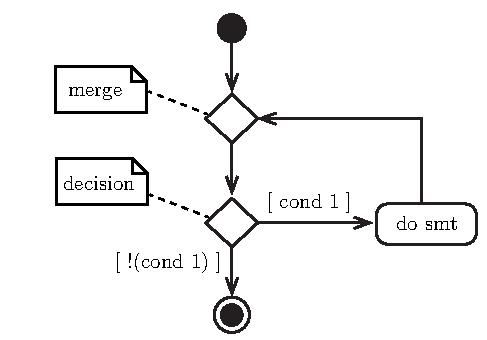
\includegraphics[width=0.50\linewidth]{01_Basics/figures/uml/IterationStatement-00-UML-while.pdf}
% \captionof{figure}{UML \texttt{while} Activity Diagram Representation}
% \label{fig:ch01_Basics_UML_IterationStatement-00-while}
% %~\ref{fig:ch01_Basics_UML_IterationStatement-00-while} 
% %%%%%%%%%%%%%%%%%%%%%%%%%%End figure
% \end{minipage}
% \begin{minipage}{.25\textwidth}
% %%%%%%%%%%%%%%%%%%%%%%%%%%%%%%%%%Begin code
% \begin{lstlisting}[frame=tlrb,numbers=none,mathescape=true,escapechar=\%,columns=flexible]
% some awesome code here
% \end{lstlisting}
% %%%%%%%%%%%%%%%%%%End Code
% \end{minipage}
% \vspace{0.5cm}
% %end minipages


%\begin{enumerate}
%	\item Initialize timer and directions registers
%    \item Specify initial state
%    \item Perform FSM controller
%   \begin{enumerate}
%    	\item Call an output function, which depends on the state
%        \item Delay, which depends on the state
%        \item Call an input function to get the status of the coin sensors
%        \item Change states, which dependes on the state and the input
%    \end{enumerate}
%\end{enumerate}

% \begin{enumerate}
% 	\item Current instruction is finished,
%     \item Eight registers are pushed on the stack,
%     \item LR is set to 0xFFFFFFF9,
%     \item IPSR is set to the interrupt number,
%     \item PC is loaded with the interrupt vector
% \end{enumerate}

% Itemize categoriza poniendo (.) en lugar de números
% \begin{itemize} 
% 	\item I
% 	\item I
% 	\item Y
% 	\item Y
% 	\item Y
% 	\item Y
% 	\item 
% \end{itemize}

% \begin{table}[!h]
% \centering
% \begin{tabular}{|l|l|l|} \hline
% $p$ & bit Field & Interrupt         \\\hline
% $3$ & \bitsRange[31]{29} & Interrupt [$4m+3$]  \\\hline
% $2$ & \bitsRange[23]{21} & Interrupt [$4m+2$]  \\\hline
% $1$ & \bitsRange[15]{13} & Interrupt [$4m+1$]  \\\hline
% $0$ & \bitsRange[7]{5} & Interrupt [$4m$]   \\\hline
% \end{tabular}
% \caption{pasteCaption}
% \label{tab:t_rt_ch04_}
% ~\ref{tab:t_rt_ch04_}
% \end{table}

% Insertar URL
%\url{https://www.osha.gov/Publications/laboratory/OSHAfactsheet-laboratory-safety-noise.pdf}\\
%\href{}{}

% \newcommand{\bitsRange}[2][50]{\texttt{{#1}-{#2}}}
% \newcommand{\CustomHex}[2][0000]{\texttt{0x{#1}.{#2}}}
% \newcommand{\GPIOPort}[1]{\texttt{GPIO\_PORT{#1}}}
% \newcommand{\GPIOPortR}[2][A]{\texttt{GPIO\_PORT{#1}\_{#2}\_R}}
% \newcommand{\GPIOPortHandler}[1]{\texttt{GPIO\_PORT{#1}\_Handler}}
% \newcommand{\HandlerISR}[1]{\texttt{#1\_Handler}}
% \newcommand{\IRQnr}[1]{\texttt{{#1}}}
% \newcommand{\NVICPRI}[1]{\texttt{NVIC\_PRI{#1}\_R}}
% \newcommand{\NVICEN}[1]{\texttt{NVIC\_EN{#1}\_R}}
% \newcommand{\NVICDIS}[1]{\texttt{NVIC\_DIS{#1}\_R}}
% \newcommand{\Ttimer}[2][A]{\texttt{Timer\_{#2}{#1}}}
% \newcommand{\xNrbit}[1]{$#1$-\texttt{bit}}
% \newcommand{\xNrbits}[1]{$#1$-\texttt{bits}}
% \newcommand{\camouflagegreenCellColor}{\cellcolor[rgb]{0.47, 0.53, 0.42}}
% \newcommand{\lavenderCellColor}{\cellcolor[rgb]{0.9, 0.9, 0.98}}
% \newcommand{\volties}[2][0]{$\si{{#1}\volt}_{#2}$}
% \newcommand{\volti}[1]{$\si{{#1}\volt}$}
% \newcommand{\voltiposi}[1]{$+\si{{#1}\volt}$}
% \newcommand{\voltinega}[1]{$-\si{{#1}\volt}$}